\section{Tests and preliminary results}

\subsection{Pilot instance space and SA versus GR}

The pilot contains 12 configurations with two replicas (24 request instances),
each paired with three fleets (72 solver cases). It uses 200, 500, or 1000
requests; peak standard deviations of 15 or 30 minutes; tight or loose
time-window settings; and fleets at 10\%, 20\%, or 30\% of request count.
The instance-space plot shows the two time-window groups and colours cases by
the SA-to-GR ratio. The documented gap is tied to having only two levels on
this axis; the full design uses continuous ranges \tagprop.

\begin{figure}[H]
\centering
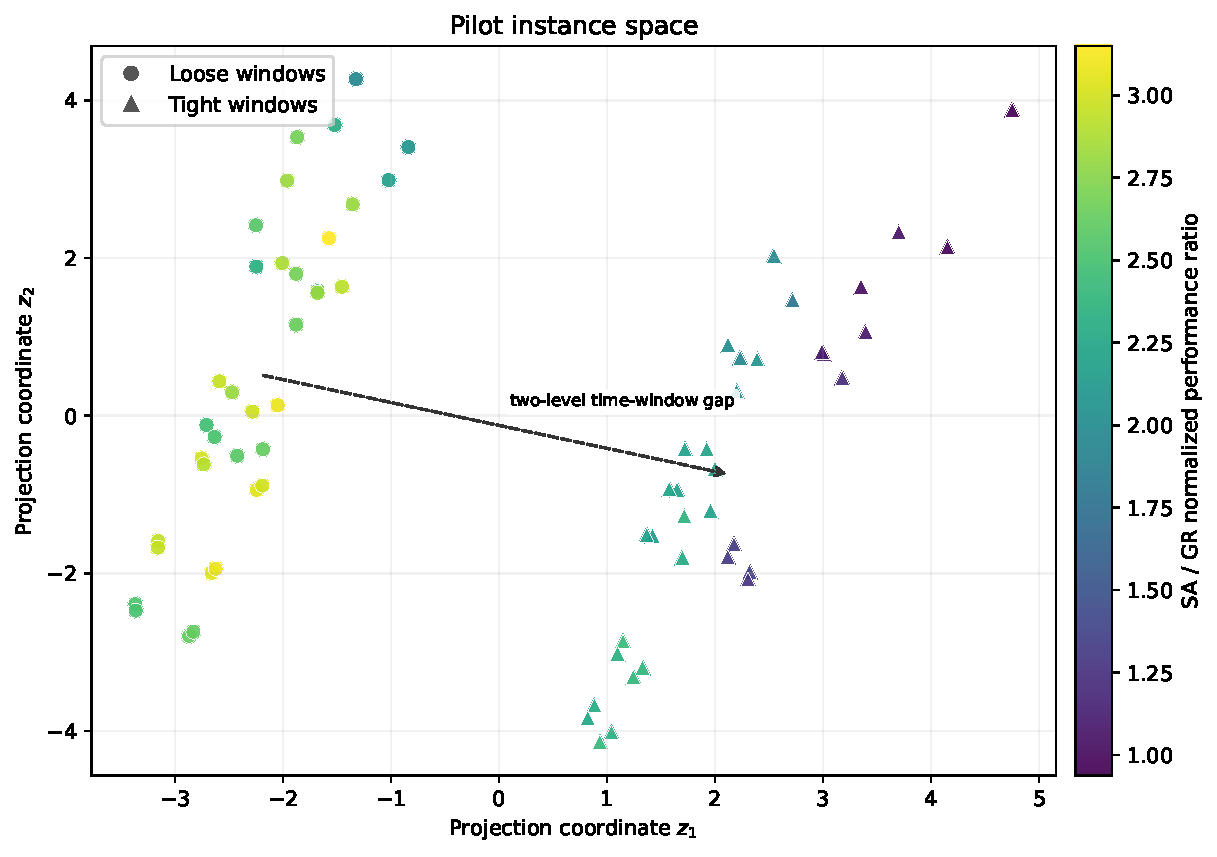
\includegraphics[width=0.88\linewidth]{figures/instance_space.pdf}
\caption{Pilot projection \texttt{z1}--\texttt{z2}. Colour is the SA/GR ratio of
the normalized performance values (above 1 favours SA); marker shape separates
tight and loose time windows. The arrow marks their centroid separation and
the two-level time-window gap. Data: \sourcepath{pilot/work/results/instance_space.csv}
and \sourcepath{pilot/work/results/perf_matrix.csv}.}
\end{figure}

Across all cases, SA is better on 70 of 72. GR is competitive only for tight
windows with the smallest fleet (8 of 72). This one-sided result may make the
pilot's algorithm-selection story thin. Whether it persists in the wide design
is \tagopen[A6].

\begin{figure}[H]
\centering
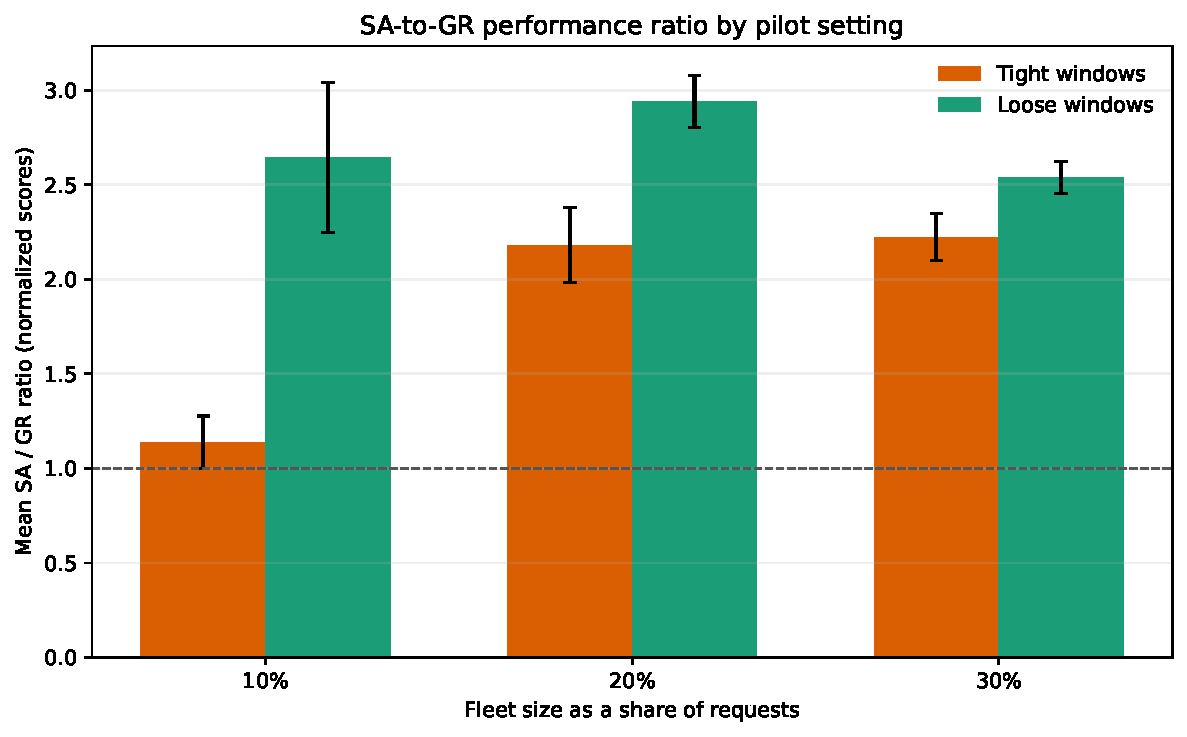
\includegraphics[width=0.78\linewidth]{figures/sa_gr_ratio.pdf}
\caption{Mean SA/GR normalized performance ratio by pilot time-window setting
and fleet size; error bars show one standard deviation across 12 cases in each
group. A ratio above 1 favours SA. Data:
\sourcepath{pilot/work/results/perf_matrix.csv}.}
\end{figure}

The seed issue is documented as 6 distinct \texttt{od\_distance\_mean} values
before the fix and 24 after it. The available pre-fix-labelled file has only
24 rows and 3 distinct values; the other 72-row files have 24. The pre-fix
value of 6 cannot be reproduced from these files, so no before/after bar chart
is shown. The post-fix value of 24 is present in
\sourcepath{pilot/work/results/features.csv}.

\subsection{Model checker and exact model}

The checker compared the original and rewritten models with the heuristic
feasibility rules in 11 scenarios. The original model mismatched in 9; v2
mismatched in none. The documented v1 defects were construction infeasibility,
capacity effectively \texttt{C-2}, shifted travel-time columns, no third-party
option, and an objective inconsistent with the heuristic.

\begin{table}[H]
\centering
\small
\caption{Exact model v2 on small instances. First-run values are from the
available raw record before valid ride lower bounds and other improvements.
Rerun figures are reported by session in \sourcepath{docs/02_tests_and_results.md};
the rerun objective and bound were not tabulated there.}
\begin{tabularx}{\linewidth}{@{}l l r r r r X@{}}
\toprule
Requests & Run & Objective & Bound & Gap & Time (s) & Result\\
\midrule
5 & First & 7284.99 & 170.376 & 97.66\% & 3600.02 & Time limit\\
5 & Rerun & Not tabulated & Not tabulated & 0\% (optimal) & 2.5 & Optimal after valid ride lower bounds\\
10 & First & 16261 & 0 & 100\% & 3600.07 & Time limit\\
10 & Rerun & Not tabulated & Not tabulated & 25\% & 3600 limit & Gap reported at limit\\
15 & First & 39034 & 0 & 100\% & 3600.35 & Time limit\\
15 & Rerun & Not tabulated & Not tabulated & Not reported & 3600 limit & Not solved to optimality\\
\bottomrule
\end{tabularx}
\end{table}

\noindent\textit{Table note:} Rerun status, gap, and five-request time are
reported by session; no rerun raw log is identified in the source. First-run
objective, bound, gap, and time are transcribed from
\sourcepath{pilot/work/v2_tests/v2_results.txt}. The \SI{3600}{s} rerun limits
for 10 and 15 requests follow the documented one-hour limit; a precise
termination time is not given. SA was reported as 4.6\% above v2's proven
five-request optimum and at least 20\% above the unproven ten-request v2
solution. A full SA/v2 objective-and-vehicle table is \tagopen[A5].

\subsection{Generation profile}

The six-request profile took 250 seconds wall time and 192 seconds CPU before
the cache. Nearest-node lookup accumulated 117.8 seconds of the 154.3-second
request phase; imports took about 60 seconds and the request plot about
27 seconds. After the fix, the whole run took 115 seconds wall time and 72
seconds CPU. The reported post-fix maximum memory of 67 MB is suspicious and
must not be used for sizing \tagopen[G6].

\begin{figure}[H]
\centering
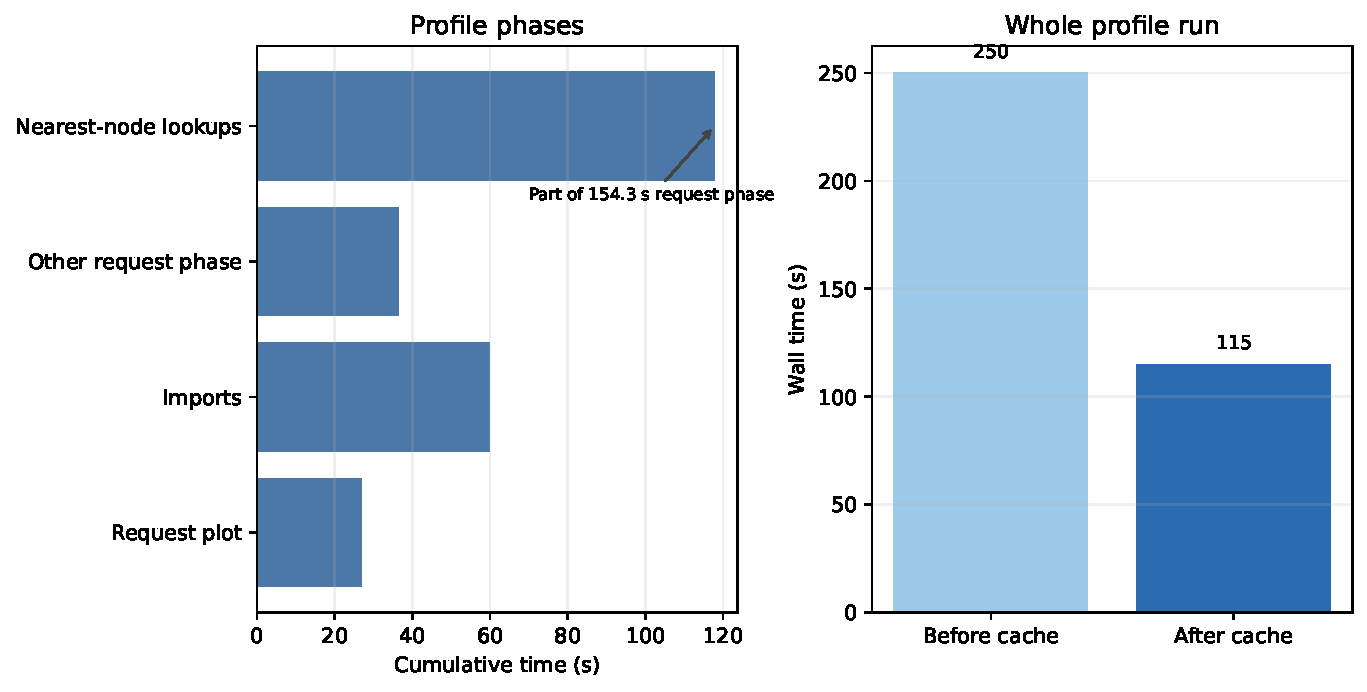
\includegraphics[width=0.78\linewidth]{figures/generation_profile.pdf}
\caption{Measured generation costs before the nearest-node cache and total
wall time before/after it. The nearest-node bar is part of the full request
phase, not an additional phase. After-fix total uses the documented 115 s
measurement. Source: \sourcepath{docs/02_tests_and_results.md}, T7.}
\end{figure}

\subsection{Network build and resource use}

The region network contains 3515 stations, with none on Bornholm. The build
used one core and ran for 3.4 hours while waiting on Overpass for part of the
time. A separate generation job with a station matrix had used 7.1 GB of an
8 GB reservation after 5.3 hours and had written no output files. The eventual
job result is \tagopen[G1]; the unaccounted time is \tagopen[G3].

\begin{table}[H]
\centering
\small
\caption{Recorded HPC resource use. Reserved memory is per slot. Missing or
unmeasured values are marked rather than estimated.}
\begin{tabularx}{\linewidth}{@{}p{0.20\linewidth}p{0.10\linewidth}p{0.14\linewidth}p{0.12\linewidth}p{0.15\linewidth}p{0.14\linewidth}@{}}
\toprule
Phase & Cores & Reserved & Used & CPU use & Runtime\\
\midrule
Network build & 1 & 6 GB & 4466 MB & 28\% & 12374 s (3.4 h)\\
6-request profile, before fix & 1 & 8 GB & 1593 MB & 77\% & 250 s\\
6-request profile, after fix & 1 & 8 GB & 67 MB\textsuperscript{a} & 63\% & 115 s\\
218-request generation test & 1 & 8 GB & 7.1 GB & About 1 core & 5.3 h, unfinished\\
SA/GR pilot solver & 1 & 16 GB & About 6 GB & Not reported & Not reported\\
Exact model v2 & 4 threads\textsuperscript{b} & Not stated & Not stated & Not stated & 1 h limit\\
\bottomrule
\end{tabularx}
\end{table}

\noindent\textsuperscript{a}The 67 MB maximum is identified as suspicious in the
source. \textsuperscript{b}The first-run raw logs show four threads; the HPC
resource table says the exact-model resource size is not yet established.
The exact-model rerun status and timing are reported by session. For network
and profile measurements, values are transcribed from the documented
measurements; the raw session logs are not all identified. Do not treat
unreported solver CPU use or runtime as zero.
